\documentclass[11pt,a4paper]{article}
\usepackage[T1]{fontenc}
\usepackage{lmodern}
\usepackage[a4paper,left=22mm,right=22mm,top=20mm,bottom=20mm,includeheadfoot]{geometry}
\usepackage{fancyhdr}
\usepackage[utf8]{inputenc}
\usepackage{amsmath,amssymb,amsthm,mathtools}
\usepackage[protrusion=true,expansion=false]{microtype}
\usepackage{booktabs,tabularx,array,longtable,multirow}
\usepackage{enumitem}
\usepackage{listings}
\usepackage{tikz}
\usetikzlibrary{arrows.meta,positioning,calc,fit}
\usepackage{graphicx}
\usepackage{hyperref}
\usepackage{xcolor}
\usepackage{url}
\usepackage{float}
\usepackage{placeins}
\usepackage{etoolbox}

\definecolor{docblue}{HTML}{203A5F}
\definecolor{docaccent}{HTML}{2F6B92}
\definecolor{docgreen}{HTML}{2F7358}
\definecolor{docwarm}{HTML}{9A5A2B}
\definecolor{docpale}{HTML}{F6F8FA}
\hypersetup{colorlinks=true,linkcolor=docblue,citecolor=docblue,urlcolor=docaccent,pdfauthor={Rituraj Basak},pdftitle={Dependency-Oriented Computation: Persistent-Graph Semantics for Incremental Repair}}
\setlist{nosep,leftmargin=1.4em}
\lstset{basicstyle=\ttfamily\footnotesize,columns=fullflexible,frame=single,framerule=0.3pt,breaklines=true,aboveskip=4pt,belowskip=4pt}

\newtheoremstyle{docstyle}{4pt}{4pt}{\itshape}{}{\bfseries}{.}{0.45em}{}
\theoremstyle{docstyle}
\newtheorem{theorem}{Theorem}
\newtheorem{lemma}{Lemma}
\newtheorem{corollary}{Corollary}
\newtheorem{definition}{Definition}
\newtheorem{principle}{Principle}
\newtheorem{boundary}{Boundary}
\newcommand{\same}{\operatorname{same}}
\newcommand{\users}{\operatorname{users}}
\newcommand{\dom}{\operatorname{dom}}
\newcommand{\src}{\mathrm{src}}
\newcommand{\Reach}{\operatorname{Reach}}
\newcommand{\Obs}{\operatorname{Obs}}
\newcommand{\DOC}{\mathrm{DOC}}
\newcommand{\botv}{\bot}
\newcommand{\R}{\mathcal{R}}
\newcommand{\N}{\mathbb{N}}

\setlength{\parindent}{1em}
\setlength{\parskip}{0.12em}
\setlength{\textfloatsep}{9pt plus 2pt minus 2pt}
\setlength{\floatsep}{8pt plus 2pt minus 2pt}
\setlength{\intextsep}{8pt plus 2pt minus 2pt}
\pagestyle{fancy}
\fancyhf{}
\fancyhead[L]{\footnotesize Dependency-Oriented Computation}
\fancyhead[R]{\footnotesize \thepage}
\renewcommand{\headrulewidth}{0pt}
\setlength{\headheight}{13.6pt}
\newcommand{\keywords}[1]{\par\smallskip\noindent\textbf{Keywords:} #1\par}
\newif\iffullvisuals
\fullvisualstrue
\title{\textbf{Dependency-Oriented Computation:}\\Persistent-Graph Semantics for Incremental Repair}
\author{Rituraj Basak\\\small Independent Researcher, India\\\small \href{mailto:ycantistudy@gmail.com}{ycantistudy@gmail.com} \;\textperiodcentered\; ORCID: \href{https://orcid.org/0009-0002-7347-7064}{0009-0002-7347-7064}}
\date{}
\begin{document}
\maketitle
\begin{abstract}
Dependency-Oriented Computation (DOC) models long-lived incremental programs as a persistent finite graph of typed logical states and deterministic local definitions. For the finite kernel, a program is $G=(S,\Delta)$ and a repair configuration is $Q=(\nu,A)$, where $\nu$ is the retained valuation and $A$ is the transient set of derived states that may require reconsideration after a source update. A repair step selects any nonempty subset of the dependency-minimal active frontier, evaluates all selected definitions from one settled pre-valuation, and atomically publishes changed conclusions. A sound equality predicate may stop propagation; an always-false predicate remains correct and performs more work.

For finite acyclic programs, DOC proves termination of every legal repair schedule, uniqueness of the stable valuation, agreement with complete topological reevaluation, schedule independence, a per-episode at-most-once evaluation bound, and dependency-local repair. Recurrence, immutable graph-version replacement, logical availability, placement, and fail-stop reconstruction are stated separately with additional contracts rather than inferred from the finite theorem. A C++20 witness and five bounded model checkers test the semantics against complete reevaluation and independent oracles. In the authoritative 100-sample bare-metal campaign, sparse updates avoid most graph work and a coarse ready frontier reaches 3.544$\times$ speedup at four participants, while specialized caching and fine-grained negative cases delimit where the generic runtime is not competitive. The results support correctness and workload-specific cost-shape claims, not universal speedup or distributed scalability.
\keywords{dependency-oriented computation, incremental computation, persistent dependency graphs, parallel evaluation, dataflow, recurrence}
\end{abstract}

\section{Introduction}\label{sec:intro}
Many long-lived programs repeatedly compute almost the same result. A compiler receives another edit, a build receives another file change, and a maintained query receives another transaction. The central execution question is therefore not only how to evaluate a program once, but how to preserve justified results and repair only the part whose premises may have changed.

This paper studies that problem through an explicit persistent dependency graph. A \emph{state} is a stable logical identity with a typed value. A \emph{source} receives an environmental fact. A \emph{derived state} is produced by one local definition from an ordered sequence of premise states. A \emph{persistent conclusion} means the currently retained value of a derived state together with its logical identity; it remains reusable only while the dependency semantics continues to justify it.

\subsection{Running example and repair problem}
Consider four logical states:
\begin{lstlisting}
source a = 2
source b = 3
sum     = add(a, b)
doubled = multiply(sum, 2)
\end{lstlisting}
The premise occurrences induce Fig.~\ref{fig:running}. Initial evaluation materializes \texttt{sum = 5} and then \texttt{doubled = 10}. Suppose one atomic source batch later installs \texttt{a := 4} and \texttt{b := 1}. Only \texttt{sum} is directly invalidated. Recomputing \texttt{sum} again yields $5$. If the runtime can prove that the new value equals the retained value, propagation stops and \texttt{doubled = 10} remains justified without reevaluation. If equality cannot be proved cheaply, the runtime may conservatively reevaluate \texttt{doubled}; the final value is unchanged.

\begin{figure}[t]
\centering
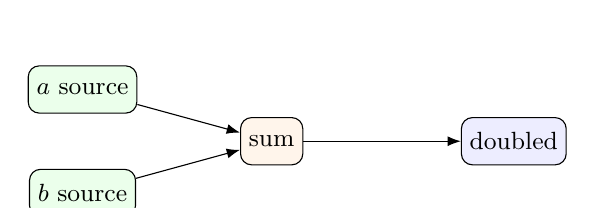
\begin{tikzpicture}[>=Latex,node distance=12mm and 18mm,every node/.style={draw,rounded corners,minimum height=6mm,inner sep=3pt,font=\small}]
\node[fill=green!8] (a) {$a$ source};
\node[fill=green!8,below=7mm of a] (b) {$b$ source};
\node[fill=orange!8,right=20mm of $(a)!0.5!(b)$] (s) {sum};
\node[fill=blue!7,right=20mm of s] (d) {doubled};
\draw[->] (a) -- (s); \draw[->] (b) -- (s); \draw[->] (s) -- (d);
\end{tikzpicture}
\caption{The running program. Premise occurrence induces the dependency graph used both for evaluation order and later repair.}\label{fig:running}
\end{figure}

This small example contains the finite mechanism. The program graph persists. The valuation persists. A source batch creates a temporary set of repair obligations. The next eligible work is determined from dependency order rather than from a separately maintained invalidation or scheduling graph. Equality cutoff is an optimization of propagation, not a correctness requirement.

\subsection{Problem statement}
The finite problem addressed here is: given a persistent finite acyclic graph, retained values from a previous stable point, and a validated source update, define a repair relation that (i) never observes an inconsistent intermediate result, (ii) permits any dependency-respecting sequential or parallel schedule, (iii) terminates, and (iv) reaches the same result as complete reevaluation. Section~\ref{sec:core} gives that relation; Section~\ref{sec:meta} proves its properties.

Real compilers and build systems invoke fallible tools, interact with files and processes, and perform effects. Within the finite kernel, such behavior must either be made explicit in the value domain (for example, a typed success/error result) while the local transformation remains total and deterministic, or remain outside the kernel behind an explicit effect or recovery boundary. Section~\ref{sec:assumptions} states these assumptions before the semantics is used.

\subsection{Scope and technical contribution}
DOC does not claim that dependency graphs, incremental repair, demand, caching, or parallel evaluation are individually new. The contribution evaluated here is the particular finite factorization around a declared persistent logical-state graph $G=(S,\Delta)$, a retained valuation $\nu$, an explicit repair-obligation set $A$, and one frontier-subset transition. The same rule covers first materialization and later repair; the dependency-minimal frontier supplies legal independent work; and sound one-way equality cutoff can reduce propagation without becoming part of the semantic equality relation.

The closest prior models often make different representational choices. Self-adjusting computation records and updates dynamic dependence structures produced by execution; Adapton adds demand to an incremental computation graph; build-system models separate scheduling and rebuilding components; differential/timely dataflow use richer version or timestamp structures for iterative distributed dataflow. Section~\ref{sec:related} compares these choices directly rather than claiming historical priority for dependency tracking itself.

\subsection{Semantic boundary}
A DOC local definition may be arithmetic, pattern matching, a query operator, a vector kernel, a verified routine, or another deterministic host function. DOC specifies the global relation among persistent states: which conclusions are justified, which states become repair obligations, what work is ready, when a repair episode is stable, and what stable value may be observed. It does not prescribe one universal syntax for the internals of every local function. When internal structure matters for reuse or parallelism, a coarse definition can be replaced by a finite boundary-equivalent DOC expansion; an implementation may also physically fuse logical definitions when observations are preserved.

\section{Model intuition and contributions}
DOC separates logical meaning from physical mechanisms that may vary without changing it. Table~\ref{tab:claimmap} states what is proved, what is conditional on additional contracts, and what is supported only by implementation or measurements.

\begin{table}[t]
\centering\footnotesize
\caption{Claim and evidence map.}\label{tab:claimmap}
\begin{tabularx}{\textwidth}{@{}p{.18\textwidth}X p{.28\textwidth}@{}}
\toprule Layer & Contains & Status\\ \midrule
Finite core & $G=(S,\Delta)$, valuation, active set, source batch, frontier-subset transition, observation & Proved; implemented; differentially and exhaustively checked in bounded domains\\
Versioned recurrence & Epoch templates, carry bindings, finite demanded prefixes, retention, divergence, universality argument & Defined extension; finite-prefix execution implemented\\
Immutable graph versions & $G_k\to G_{k+1}$, stable names, semantic compatibility, private validation and atomic commit & Defined extension; checked against from-scratch evaluation\\
Safe realization & Private evaluation, immutable publication, protected reads, roots, reclamation & Normative contract; typed object-store witness\\
Placed realization & Resources, logical roles, transport, generations, join, drain, bounded fail-stop reconstruction & Conditional theorem; executable loopback witness\\
Policy boundaries & Fixed points, conflict/replica policy, partitions, retention, irreversible effects & Explicit policy; not inferred from dependency\\ \bottomrule
\end{tabularx}
\end{table}

The status distinctions are exact: \emph{proved core} means a theorem about the finite relation; \emph{defined extension} means additional semantics stated separately; \emph{realization contract} means physical obligations required to preserve observation; \emph{executable evidence} means tested behavior of one implementation; and \emph{remaining boundary} means policy or physics that dependency cannot determine by itself.

\section{Standing assumptions and scopes}\label{sec:assumptions}
The assumptions are collected here so later definitions and results need not restate them. They are also an applicability checklist for compilers, build systems, and other motivating applications: fallible external tools must be represented as explicit values or placed outside the pure finite kernel.

The abstract finite transition rule itself needs no scheduler-fairness premise: every transition selects a nonempty ready subset, and the acyclic work argument bounds the number of selections. Fairness appears only in physical progress claims that allow work or reclamation to be postponed by a runtime.

For a compiler or build system, purity and totality are modeling obligations rather than claims that external tools never fail. File contents, command-line arguments, tool versions, configuration, and other relevant environmental facts can be explicit source values. A fallible deterministic tool result can be represented as a typed value if the invocation is fully determined by those premises. Nondeterministic process execution, network calls, authorization, and irreversible actions instead occur outside the finite local transformation; their committed outcome becomes a later source fact.

\begin{table}[t]
\centering\scriptsize
\caption{Standing assumptions by semantic scope. Only the finite-kernel row is assumed by the central stabilization theorem.}\label{tab:assumptions}
\begin{tabularx}{\textwidth}{@{}p{.18\textwidth}X@{}}
\toprule Scope & Assumptions\\ \midrule
Finite kernel & Finite state family and premise sequences; acyclic dependency graph; pointwise-typed, pure, deterministic, total, terminating local transformations; typed source batches; sound cutoff predicates, which may conservatively return false; repair-admissible seed.\\
Sources, failures, effects & Environmental nondeterminism enters through committed source batches. Recoverable absence/failure is represented inside a value domain. Host exceptions, cancellation, authorization, and irreversible actions are outside ordinary local transformations.\\
Versioned recurrence & Each epoch satisfies the finite assumptions; carry is typed, single-authority, and forward in logical time; uncarried sources receive explicit facts/defaults; completed observations demand finite prefixes.\\
Graph versions & Candidate graph is well formed and stabilized privately. Reuse requires stable identity, same role/domain/equality, and explicit observational compatibility before atomic commit.\\
Physical realization & Observation occurs only at committed stable boundaries; captured values remain protected; reclamation/transport/join/drain/recovery claims require their stated progress and quiescence conditions.\\ \bottomrule
\end{tabularx}
\end{table}

\section{Core semantics}\label{sec:core}
The finite logical kernel proceeds from program objects and satisfaction to initialization, source updates, the ready frontier, and a single repair transition. Mathematical consequences are separated from extensions, realization obligations, and empirical performance evidence.

\subsection{Basic objects and satisfaction}
A finite DOC program is
\begin{equation}G=(S,\Delta),\label{eq:program}\end{equation}
where $S$ is a finite family of stable logical state identities and $\Delta$ is a partial map whose domain contains exactly the derived states. Every $s\in S$ has a declared value domain $V_s$. Physical addresses, workers, and storage locations are not elements of $S$.

\begin{definition}[State]\label{def:state}
A state is a stable logical identity $s\in S$ with value domain $V_s$. Its identity is independent of a memory address, thread, process, machine, or storage location.
\end{definition}
A state may currently be unmaterialized. Each $V_s$ has its ordinary semantic equality. A realization may additionally provide a total decidable cutoff predicate
\begin{equation}
\same_s:V_s\times V_s\to\mathrm{Bool},\qquad \same_s(x,y)=\mathrm{true}\Rightarrow x=y.
\label{eq:cutoff}
\end{equation}
The implication is the only soundness requirement: the predicate may conservatively return false even for equal values. The always-false predicate is therefore valid and yields complete propagation without cutoff. Hash-only or tolerance tests are invalid unless returning true proves equality in the declared value domain.

\begin{definition}[Local definition]\label{def:local}
For each derived state $d$, let $P_d=(s_1,\ldots,s_k)$ be its ordered premise sequence. The partial map stores $\Delta(d)=(P_d,f_d)$ where
\[
f_d:V_{s_1}\times\cdots\times V_{s_k}\to V_d
\]
is a local transformation satisfying the finite-kernel assumptions.
\end{definition}
The conclusion is the map key $d$ itself. Zero-premise definitions represent constant derived states. Let
\begin{equation}D=\dom(\Delta),\qquad S_{\src}=S\setminus D.\label{eq:partition}\end{equation}
States in $D$ are derived; states outside $D$ are sources. Single-producer authority follows from the partial-map representation. A state $x$ is a direct premise of $d$ when $x$ occurs in $P_d$; users are induced rather than separately declared:
\begin{equation}\users(x)=\{d\in D\mid x\text{ occurs in }P_d\}.\label{eq:users}\end{equation}

A valuation is pointwise typed,
\begin{equation}\nu(s)\in V_s\cup\{\botv\}\quad\text{for every }s\in S,\label{eq:valuation}\end{equation}
where $\botv$ means no current materialization, not application-level null, deletion, failure, or unknown data. For $P_d=(s_1,\dots,s_k)$, let $\nu(P_d)$ denote componentwise lookup of those premises. If $\Delta(d)=(P_d,f_d)$, then $d$ is locally satisfied when all premises are materialized and
\begin{equation}\nu(d)=f_d(\nu(P_d)).\label{eq:satisfaction}\end{equation}
Local satisfaction uses equality in the value domain. The operational cutoff predicate is separate: it may fail to recognize equality but must never claim sameness for unequal values.

An observation requests the stable value of a logical state. The finite rule is stated for whole-graph epochs; demand-restricted execution applies the same rule to the ancestor-closed induced subprogram of the requested state with materialized boundary sources.

\subsection{Computational expansion}
\begin{definition}[Expansion]\label{def:expansion}
If $\Delta(d)=(P,f_d)$, an expansion replaces it by a finite pure acyclic DOC subgraph that reads the same boundary premises $P$, publishes to the same boundary state $d$, uses fresh internal identities, and yields $f_d$ for every typed boundary tuple.
\end{definition}
Expansion is a semantic granularity choice, not an obligation to schedule every primitive separately; a realization may physically fuse or batch an expanded region while retaining logical boundaries.

\iffullvisuals
\begin{figure}[t]
\centering
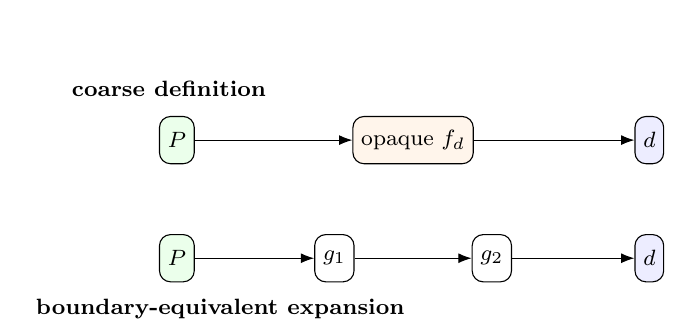
\begin{tikzpicture}[>=Latex,every node/.style={draw,rounded corners,minimum height=6mm,inner sep=3pt,font=\footnotesize}]
\node[fill=green!8] (p1) at (0,1.0) {$P$};
\node[fill=orange!8] (f) at (3.0,1.0) {opaque $f_d$};
\node[fill=blue!7] (d1) at (6.0,1.0) {$d$};
\draw[->] (p1)--(f); \draw[->] (f)--(d1);
\node[draw=none,font=\footnotesize\bfseries] at (-0.1,1.65) {coarse definition};
\node[fill=green!8] (p2) at (0,-0.5) {$P$};
\node (g1) at (2.0,-0.5) {$g_1$};
\node (g2) at (4.0,-0.5) {$g_2$};
\node[fill=blue!7] (d2) at (6.0,-0.5) {$d$};
\draw[->] (p2)--(g1); \draw[->] (g1)--(g2); \draw[->] (g2)--(d2);
\node[draw=none,font=\footnotesize\bfseries] at (0.55,-1.15) {boundary-equivalent expansion};
\end{tikzpicture}
\caption{Expansion replaces one coarse definition by a finite DOC subgraph with the same premises and boundary result; the two rows are alternatives, not sequential stages.}\label{fig:expansion}
\end{figure}
Figure~\ref{fig:expansion} illustrates that refinement. Physical implementations may still fuse or batch the expanded region.
\fi

\subsection{Initial and later stabilization}
Initially, sources are present, derived states are absent, and every definition is active. In the running example, \texttt{sum} evaluates to $5$ and then \texttt{doubled} to $10$. After the atomic batch \texttt{a := 4, b := 1}, \texttt{sum} is reconsidered and again produces $5$. Under exact cutoff, the retained equality is proven and \texttt{doubled} is not activated. Under always-propagate cutoff, it harmlessly reevaluates to $10$. First materialization and later repair therefore differ only in what is already retained.

\iffullvisuals
\begin{figure}[t]
\centering
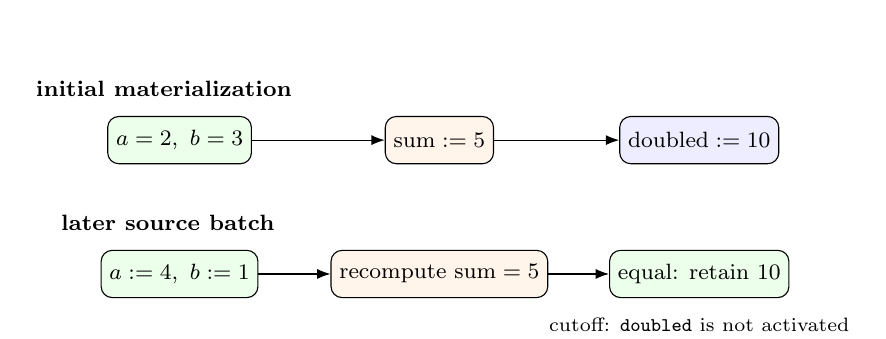
\begin{tikzpicture}[>=Latex,every node/.style={draw,rounded corners,minimum height=6mm,inner sep=3pt,font=\footnotesize}]
\node[draw=none,font=\footnotesize\bfseries] at (-0.2,1.55) {initial materialization};
\node[fill=green!8] (i1) at (0,0.9) {$a=2,\ b=3$};
\node[fill=orange!8] (i2) at (3.3,0.9) {$\mathrm{sum}:=5$};
\node[fill=blue!7] (i3) at (6.6,0.9) {$\mathrm{doubled}:=10$};
\draw[->] (i1)--(i2); \draw[->] (i2)--(i3);
\node[draw=none,font=\footnotesize\bfseries] at (-0.15,-0.15) {later source batch};
\node[fill=green!8] (u1) at (0,-0.8) {$a:=4,\ b:=1$};
\node[fill=orange!8] (u2) at (3.3,-0.8) {recompute $\mathrm{sum}=5$};
\node[fill=green!8] (u3) at (6.6,-0.8) {equal: retain $10$};
\draw[->] (u1)--(u2); \draw[->] (u2)--(u3);
\node[draw=none,font=\scriptsize] at (6.6,-1.45) {cutoff: \texttt{doubled} is not activated};
\end{tikzpicture}
\caption{Initial materialization and later repair use the same stabilization relation. Retained equality stops the later wave.}\label{fig:repair-example}
\end{figure}
Figure~\ref{fig:repair-example} makes the reuse boundary explicit: the later epoch differs only in the stable values already retained.
\fi

\subsection{Finite active-set transition system}
With $G$ fixed, the operational configuration is
\begin{equation}Q=(\nu,A),\qquad A\subseteq D.\label{eq:config}\end{equation}
$\nu$ persists across epochs; $A$ is transient and records repair obligations. Membership in $A$ does not assert that the retained value is unequal. A configuration is \emph{repair-admissible} when every source is materialized and every inactive derived state is materialized and locally satisfied:
\begin{equation}
(\forall s\in S_{\src}:\nu(s)\neq\botv)\ \land\ (\forall d\in D\setminus A:\nu(d)\neq\botv\land d\text{ is locally satisfied}).
\label{eq:admissible}
\end{equation}
A quiescent configuration has $A=\varnothing$; a repair-admissible quiescent configuration is exactly a stable valuation.

Write $e\prec d$ when derived state $e$ is a transitive premise of $d$. The ready frontier is
\begin{equation}R(A)=\{d\in A\mid \nexists e\in A:e\prec d\}.\label{eq:ready}\end{equation}
Every ready definition has materialized premises; distinct frontier members cannot depend on one another and have distinct conclusions.

For a total typed source environment $I$, initialization sets
\begin{equation}
\nu_0(s)=\begin{cases}I(s),&s\in S_{\src},\\\botv,&s\in D,\end{cases}\qquad A_0=D.
\label{eq:init}
\end{equation}
For a validated finite typed source batch $U_b$, let
\begin{equation}
X=\{s\in\dom(U_b)\mid \same_s(U_b(s),\nu(s))=\mathrm{false}\}.
\label{eq:changed}
\end{equation}
The post-boundary seed is
\begin{align}
\nu_0&=\nu[s\mapsto U_b(s)\text{ for }s\in X],\label{eq:updateval}\\
A_0&=A\cup\bigcup_{s\in X}\users(s).\label{eq:updateactive}
\end{align}
Assignments in $X$ are installed atomically; direct users are added to any obligations already present. The step preserves repair admissibility.

Choose any nonempty finite $F\subseteq R(A)$. For each $d\in F$ with $\Delta(d)=(P_d,f_d)$, evaluate privately from the same pre-transition valuation:
\begin{equation}v_d=f_d(\nu(P_d)).\label{eq:candidate}\end{equation}
Define the propagating-conclusion set
\begin{equation}
C_F=\{d\in F\mid \nu(d)=\botv\}\cup\{d\in F\mid \nu(d)\neq\botv\land\same_d(v_d,\nu(d))=\mathrm{false}\}.
\label{eq:cf}
\end{equation}
Publish every candidate in $C_F$ as one logical commit:
\begin{align}
\nu'&=\nu[d\mapsto v_d\text{ for }d\in C_F],\label{eq:publish}\\
A'&=(A\setminus F)\cup\bigcup_{d\in C_F}\users(d).\label{eq:nextactive}
\end{align}
Then $(\nu,A)\to(\nu',A')$. A singleton $F$ gives sequential execution; a larger $F$ gives parallel evaluation. All candidates read the same settled pre-state and the selected frontier joins before logical commit. Candidates proven equal are removed from $A$ without replacement or downstream activation. Conservative false negatives may add work but do not alter correctness. The C++20 witness chooses the complete frontier $F=R(A)$.

\begin{figure}[t]
\centering
\begin{minipage}{.94\textwidth}\small
\begin{lstlisting}
Input: fixed finite program G=(S, Delta) and repair-admissible Q=(nu,A)
1. Boundary step:
   Initial run: install source facts, derived := absent, A := D.
   Later run: validate source batch, atomically install assignments not
   proven equal, and add their direct users to A.
2. While A is nonempty:
   a. Compute R(A), active states with no active strict ancestor.
   b. Choose nonempty F subset R(A).
   c. Evaluate every d in F privately from the same committed pre-valuation.
   d. Form C_F from absent candidates or candidates not proven equal.
   e. Atomically publish C_F.
   f. Remove F from A; add users(d) for d in C_F.
3. When A is empty, expose the requested stable observation.
\end{lstlisting}
\end{minipage}
\caption{Finite DOC stabilization. The executable witness chooses the complete ready frontier.}\label{alg:finite}
\end{figure}

\begin{boundary}[Failure before publication]
Typed result/option/error values are ordinary values when the local function remains total. A thrown host callback violates the finite theorem's totality premise. Defensively, if any candidate in $F$ throws before the barrier, the witness publishes none of that frontier and keeps every state in $F$ active. Accepted source facts remain committed. Retry, rollback, and irreversible-action policy belong to the effect or recovery boundary.
\end{boundary}

\section{Central metatheory}\label{sec:meta}
\begin{lemma}[Frontier materialization and preservation]\label{lem:preservation}
In a repair-admissible configuration, every ready definition has materialized premises. An accepted source boundary step and every valid frontier-subset transition preserve repair admissibility.
\end{lemma}
\begin{proof}
Let $Q=(\nu,A)$ be repair-admissible. If $d\in R(A)$ and a premise $p$ is a source, $p$ is materialized by admissibility. If $p$ is derived and active, then $p\prec d$, contradicting readiness; if inactive, admissibility makes it materialized and locally satisfied. Thus every candidate in a valid selection is defined.

For a source batch, any derived state left inactive was inactive before and has no changed source premise; otherwise it would have been activated. Its value and premises are unchanged, so it remains materialized and satisfied. For a frontier transition, let $x$ be inactive in $A'$. If $x\in F$, its premises lie outside $F$ and are unchanged by the commit. The candidate therefore satisfies its definition; if $x\notin C_F$, cutoff soundness gives $v_x=\nu(x)$. If $x\notin F$, it was already inactive, and any selected premise that changed would place $x$ in the propagated user union, contradicting $x\notin A'$. Hence its prior satisfaction is preserved.
\end{proof}

\begin{lemma}[At-most-once selection and finite progress]\label{lem:progress}
Fix one repair episode: a repair-admissible seed followed only by frontier-subset transitions and no intervening accepted source batch. Every derived definition is selected at most once. Consequently every valid transition sequence is finite, and every maximal sequence ends quiescent.
\end{lemma}
\begin{proof}
When $d$ is selected, it has no active strict ancestor. Suppose some strict ancestor later became active and choose the first such activation. Activation can arise only from publication by one of that ancestor's direct premises. That publishing premise is itself a strict ancestor of $d$ and must have been active and selected earlier, contradicting the choice of the first later ancestor activation. Sources do not change inside the episode. Thus no strict ancestor of $d$ can publish after $d$ is selected, its premises cannot later change, and $d$ cannot be reactivated. At most $|D|$ definitions are selected; each transition selects a nonempty set. If a finite maximal sequence ended with $A\neq\varnothing$, acyclicity would give a minimal active member and hence another ready transition. Therefore a maximal sequence ends with $A=\varnothing$.
\end{proof}

\begin{lemma}[Canonical stable valuation]\label{lem:canonical}
For fixed current source values, there is exactly one stable valuation, namely complete topological reevaluation of every derived definition.
\end{lemma}
\begin{proof}
Choose a topological order of $D$. Keep each current source value and define $\mu(d)=f_d(\mu(P_d))$ in that order. Totality and typing make $\mu$ exist. Any stable valuation has the same source values; induction over the order and determinism force every derived conclusion to agree with $\mu$. Thus every stable valuation equals complete reevaluation.
\end{proof}

\begin{theorem}[Finite stabilization]\label{thm:finite}
For every well-formed finite acyclic DOC program, begin from any repair-admissible configuration and hold sources fixed during the repair episode. Every valid frontier-subset transition sequence is finite. Every maximal sequence ends in the unique stable valuation produced by complete topological reevaluation. The result is independent of eligible selections and their valid order, and sound exact cutoff does not change that result.
\end{theorem}
\begin{proof}
Lemma~\ref{lem:preservation} preserves repair admissibility. Lemma~\ref{lem:progress} makes every valid sequence finite and every maximal sequence quiescent. Quiescence together with repair admissibility makes every derived state materialized and locally satisfied, so the terminal valuation is stable. Lemma~\ref{lem:canonical} identifies it uniquely with complete reevaluation; hence all valid maximal schedules have the same result.

If $\same_d(v_d,\nu(d))$ is true, Eq.~\eqref{eq:cutoff} gives $v_d=\nu(d)$. Retaining the old materialization is therefore observationally identical to publishing the candidate. An inactive direct user sees no changed premise, while an already active user remains active. Conservative false negatives can activate additional users, but preservation and uniqueness still force the same terminal valuation.
\end{proof}

\begin{corollary}[Initial/later unity] First materialization and later reactive repair are the same stabilization relation with different retained valuations. \end{corollary}
\begin{corollary}[Semantic caching and work bound] At a stable boundary, every retained derived value is the unique correct value for its current premises. During one fixed repair episode each definition evaluates at most once. \end{corollary}
\begin{corollary}[Independent ready selections commute] Disjoint subsets of the same ready frontier may be evaluated and committed in either order or together: candidates read the same settled values, writes target distinct states, and propagated users combine by set union. \end{corollary}
\begin{corollary}[Source-update locality]\label{cor:locality} For a source batch applied at a stable boundary, no state outside the reflexive-transitive user closure $\Reach^*(X)$ is selected or modified. \end{corollary}
\begin{corollary}[Conservative cutoff] Any cutoff predicate satisfying only one-way soundness is correct. False negatives may add work but cannot alter the unique stable valuation. \end{corollary}

\begin{theorem}[Expansion preservation]\label{thm:expansion}
A finite acyclic boundary-equivalent expansion of one definition preserves stable observations over the original states.
\end{theorem}
\begin{proof}
Fix source values and compare complete reevaluation of the original and expanded graphs. Upstream original states are unchanged. The fresh internal expansion has a unique stable valuation by Theorem~\ref{thm:finite}, and boundary equivalence makes its published value at $d$ equal to $f_d$ on the same boundary premises. A topological induction over remaining original descendants gives the same value at every original state. Schedule independence extends the result from complete reevaluation to every valid stabilization schedule.
\end{proof}

\subsection{Reactivity, reuse, and parallelism}
Reactive systems are often described with subscriptions, observers, callbacks, or handlers. DOC does not require a second event graph: the users induced by $\Delta$ already state which definitions may be affected by a changed conclusion. In a chain \texttt{temperature $\to$ thermostat policy $\to$ heater command}, only the thermostat definition is activated directly by a temperature change. If the derived policy changes, the heater becomes active; if the cutoff predicate proves the policy equal to its retained value, the wave stops. Dependency is simultaneously the ordering relation, possible-impact relation, and repair path.

At a stable boundary, every retained derived value is the unique result required by current sources and local definitions. Reuse is therefore semantic rather than heuristic. The active set plays the role that manually maintained invalidation metadata often plays elsewhere, but it is transient: it says what may need reconsideration during the current source epoch and disappears when stabilization reaches quiescence.

After a small source batch, the runtime repairs the propagated descendant region rather than reevaluating every definition. With exact cutoff, work follows actual value change; with a conservative predicate, the region may be larger but remains dependency-local. Dense change may activate nearly the whole graph, expensive equality can erase savings, and if definitions are extremely cheap then bookkeeping, synchronization, and publication can dominate. DOC exposes available reuse; it cannot manufacture useful reuse where the graph and update contain none.

Parallelism has the same structural cause. The active region identifies potentially necessary work; its dependency-minimal frontier identifies independent next work. No frontier member transitively depends on another frontier member, and distinct frontier members publish distinct conclusions. A realization may process a frontier sequentially, on several granted CPU cores, accelerators, or placed resources. Synchronization implements the semantic rule: candidates read one settled pre-state, private evaluation completes before the frontier publication barrier, and failed candidates must not leak partial publication.

\iffullvisuals
\begin{figure}[t]
\centering
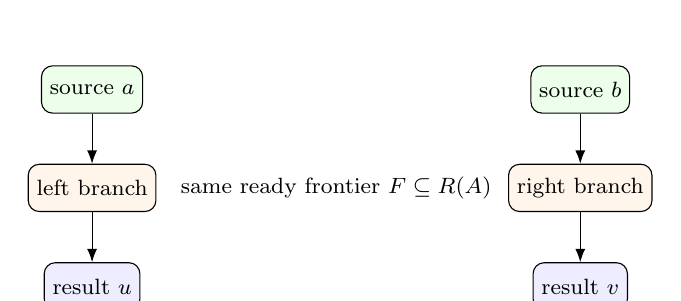
\begin{tikzpicture}[>=Latex,every node/.style={draw,rounded corners,minimum height=6mm,inner sep=3pt,font=\footnotesize}]
\node[fill=green!8] (a) at (0,1.25) {source $a$};
\node[fill=orange!8] (l) at (0,0) {left branch};
\node[fill=blue!7] (u) at (0,-1.25) {result $u$};
\node[fill=green!8] (b) at (6.2,1.25) {source $b$};
\node[fill=orange!8] (r) at (6.2,0) {right branch};
\node[fill=blue!7] (v) at (6.2,-1.25) {result $v$};
\draw[->] (a)--(l); \draw[->] (l)--(u); \draw[->] (b)--(r); \draw[->] (r)--(v);
\node[draw=none,font=\footnotesize] at (3.1,0) {same ready frontier $F\subseteq R(A)$};
\end{tikzpicture}
\caption{Independent active branches can belong to one ready frontier. No horizontal dependency connects the branches, and the program contains no worker-count syntax.}\label{fig:frontier-parallelism}
\end{figure}
Figure~\ref{fig:frontier-parallelism} shows the structural source of parallel work: readiness exposes independence before a runtime chooses any physical worker allocation.
\fi

Persistent editors, compilers, servers, simulations, dashboards, and workflows repeatedly receive partial change. DOC therefore treats temporal reuse as foundational while leaving local kernels free to use reduction-optimal, vectorized, incrementalized, or hardware-specific techniques.

\subsection{Types and provenance boundary}
Each state has a value domain $V_s$, and each definition has the typed mapping stated by $\Delta$. Types answer \emph{what values may flow here?}; dependency answers \emph{which current values justify this conclusion?}. For example, a typed syntax tree may have the same ordinary type before and after an edit, while the graph still records whether current diagnostics were derived from that tree together with the current symbol table and compiler options. In the finite active-set core, $\nu$ holds current materializations and $A$ records conclusions that may need repair during one source epoch. Ordinary result types therefore need not be parameterized by source revisions merely to support change propagation. DOC does not eliminate dependent types: value-dependent invariants remain legitimate and belong in the local language or state type system when needed.

\section{Demand restriction, recurrence, and graph evolution}\label{sec:extensions}
The proved finite kernel directly represents finite acyclic compositions. One fixed finite graph is not by itself a model of partial or unbounded computation; temporal unboundedness is obtained by composing the unchanged kernel across explicitly ordered logical epochs.

\subsection{Versioned recurrence}
Let $q_t$ denote recurrent state at epoch $t$ and let a step transformation define $q_{t+1}=T(q_t)$. Dependency points from an earlier epoch to a later one, never from a state back to itself inside the same epoch, so every materialized finite prefix remains acyclic.

\begin{definition}[Versioned recurrence]\label{def:recurrence}
A recurrent DOC program is a finite acyclic graph template indexed by logical epochs, together with an initial epoch, a demand rule, and a typed partial carry function $K:S^E_{\src}\to S^E$. If $K(s)=x$, source $s$ of epoch $t+1$ receives the value of state $x$ from epoch $t$. Each next-epoch source has at most one carry authority; every uncarried source receives an explicit epoch-local fact or fixed default. Demanding epoch $n$ instantiates and stabilizes only the finite prefix through $n$. An observation that continues demanding later epochs without reaching a stopping condition diverges.
\end{definition}

\begin{theorem}[Demand-restriction agreement]\label{thm:demand}
Let $T\subseteq S$ be finite and let $H_T$ be the ancestor-closed induced subprogram containing $T$, with each incoming boundary source materialized to the same fact as in the full program. Stabilizing $H_T$ yields exactly the restriction to $H_T$ of the unique stable valuation obtained by stabilizing the full program from those source facts.
\end{theorem}
\begin{proof}
Let $\mu$ be the unique full-program stable valuation and $\mu_T$ the unique stable valuation of $H_T$. Ancestor closure ensures that every premise of a retained derived definition is either retained or supplied as a boundary source with the same value as in $\mu$. Topological induction therefore gives $\mu_T=\mu|_{H_T}$, including every requested state.
\end{proof}

\begin{theorem}[Finite support of requested recurrence prefixes]\label{thm:recurrence}
For a finite epoch template, total local definitions, a single typed carry authority for each carried next-epoch source, and explicit facts/defaults for every uncarried source, every requested finite prefix $0,\ldots,n$ requires only finitely many template instances and finite-kernel transitions. An absorbing halt state may be reused without additional machine progress, or demand may stop at halt.
\end{theorem}
\begin{proof}
Induct on the requested epoch. Epoch zero has a finite source environment and finite acyclic graph, so finite stabilization terminates. Once epoch $t$ is stable, each carried source of epoch $t+1$ receives exactly one typed value and every other source receives its declared fact/default; the next finite instance therefore stabilizes. A finite prefix is a finite sum of finite episodes.
\end{proof}
Versioned recurrence is DOC's unbounded computational form, not an enlargement of $G$ or $Q$ for one epoch. Same-epoch fixed points require their own convergence and observation semantics and are outside the finite theorem.

\iffullvisuals
\begin{figure}[t]
\centering
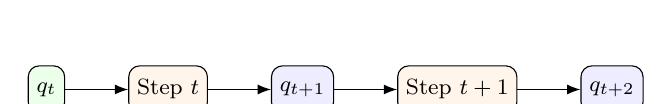
\begin{tikzpicture}[>=Latex,every node/.style={draw,rounded corners,minimum height=6mm,inner sep=3pt,font=\footnotesize},node distance=8mm]
\node[fill=green!8] (q0) {$q_t$};
\node[fill=orange!8,right=of q0] (s0) {Step $t$};
\node[fill=blue!7,right=of s0] (q1) {$q_{t+1}$};
\node[fill=orange!8,right=of q1] (s1) {Step $t+1$};
\node[fill=blue!7,right=of s1] (q2) {$q_{t+2}$};
\draw[->] (q0)--(s0); \draw[->] (s0)--(q1); \draw[->] (q1)--(s1); \draw[->] (s1)--(q2);
\end{tikzpicture}
\caption{Versioned recurrence applies the finite step transformation separately at each forward epoch, preserving acyclicity within every epoch.}\label{fig:recurrence}
\end{figure}
Figure~\ref{fig:recurrence} emphasizes that unbounded time is obtained by forward epoch construction rather than a same-epoch cycle in the finite kernel.
\fi

Iteration is repeated application of $T$. A loop state contains the variables and control location required for the next step; recursion may be represented by an explicit stack/continuation in recurrent state or demand-driven creation of later invocation states. Mutation is represented as succession of logical facts: work in epoch $t$ reads a complete value belonging to that epoch, while environmental or derived authority may publish the value used by epoch $t+1$. Multiple contributors may publish distinct proposal states, but an explicit merge/transaction/priority/lattice rule must establish authoritative state.

A deterministic two-counter machine has a finite instruction table, program counter, and two unbounded natural-number registers \cite{minsky1967}. Encode a configuration as $q_t=(\mathrm{pc}_t,r_{1,t},r_{2,t})$; one finite local \texttt{Step} definition performs the selected machine instruction and yields $q_{t+1}$.
\begin{theorem}[Universality of versioned recurrence]\label{thm:universal}
DOC with demand-driven unbounded epoch instantiation, unbounded natural values, finite case analysis, increment, zero test, and conditional decrement can simulate every deterministic two-counter machine step for step.
\end{theorem}
Mapping each machine configuration to one epoch state and the finite instruction table to finite case analysis inside \texttt{Step} gives the result by induction on $t$. A halting machine yields a finite observed prefix; a non-halting machine demands an unbounded sequence and diverges. The executable witness checks finite prefixes against a direct interpreter; that test is not a second proof of universality.

\subsection{Immutable graph-version change}
Some programs change not only source values but also which logical states and definitions exist. DOC handles this through an ordered sequence of immutable, individually well-formed graph versions $G_0\to G_1\to G_2\to\cdots$.

\begin{definition}[Graph-version commit]\label{def:graphcommit}
A commit from $G_k$ to candidate $G_{k+1}$ first stabilizes the current version and validates the candidate before reading any candidate-derived index. A current source fact crosses by stable logical name only when the candidate state remains a source with the same value domain and semantic equality. A retained derived value additionally requires the same derived authority role, an equivalence-bearing semantic key, identical ordered premise identities, and every premise to be carried or retained compatibly and remain unaffected. Domain changes, new states, or source/derived role changes are affected. The private candidate seed must be repair-admissible; its affected region is stabilized by the ordinary finite rule. The complete candidate graph and valuation replace the prior version atomically, advancing a graph-generation token.
\end{definition}
An in-flight result captured under generation $k$ may publish only while that generation remains current. Retirement removes old logical roots after active observations release them; physical reclamation then follows ordinary reachability.

A semantic key is an externally justified certificate identifier; it is not an automatic solver for function equivalence. For example, a state \texttt{tax} may retain the key \texttt{tax-rule-v3} after refactoring only when the builder compatibility process certifies the same mapping over the declared domain with unchanged ordered premise identities. A policy change to 22\% uses a different key. If compatibility cannot be established, the definition is treated as changed and repaired.

\begin{theorem}[Conditional graph-version commit agreement]\label{thm:graphcommit}
Under the stated compatibility contract, every successful commit to $G_{k+1}$ has the same stable values as constructing $G_{k+1}$ from carried current source facts and evaluating it completely from scratch. Retained compatible values change cost, not meaning.
\end{theorem}
\begin{proof}
Let $\mu^*$ be complete evaluation of $G_{k+1}$ from carried candidate sources. Same-role compatible sources agree with $\mu^*$. In candidate topological order, an inactive retained derived state may remain inactive only when its role, domain/equality, semantic key, ordered premise identities, and every premise are compatible and unaffected. Its premise values therefore equal $\mu^*$, and boundary equivalence gives the same conclusion. Hence every inactive candidate state is already materialized and locally satisfied; all others are active. The private seed is repair-admissible, so Theorem~\ref{thm:finite} converges to the unique candidate stable valuation $\mu^*$. Atomic generation commit exposes only that valuation, and stale-generation rejection prevents older work from changing it.
\end{proof}

\section{Realization contracts and boundaries}\label{sec:realization}
Authority, logical availability, and physical lifetime are not extra instructions in the finite repair rule. They are constraints on realizations that preserve the rule's observations.

\subsection{Logical availability and safe realization}
The partial-map representation gives one logical producer to every derived state. Source batches have environmental authority. Placement may move a physical executor or storage location, but it must not create a second logical producer for the same conclusion. A conforming realization evaluates candidates privately and publishes complete immutable values: a reader observes either the previous complete materialization or the next complete materialization, never a partially mutated object.

\begin{definition}[Logical availability]\label{def:availability}
A logical value is available while the program's current state, a permitted observation, retained recurrence policy, active work, or an admitted external root still entitles it to be observed or consumed. A realization preserves that availability by retaining either a usable complete materialization or sufficient authoritative information to reconstruct an observationally equivalent complete value before use.
\end{definition}
A logically available value need not remain resident in its current physical form. A realization may evict, spill, compress, deduplicate, fuse, or discard a reconstructible derived materialization. Once a value has been pinned by active observation, evaluation, publication, or transport, that complete physical object remains protected until the use finishes even if its state slot is concurrently evicted or replaced.

\iffullvisuals
\begin{figure}[t]
\centering
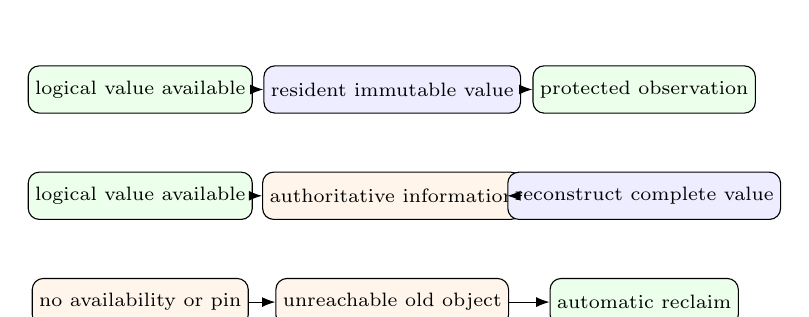
\begin{tikzpicture}[>=Latex,every node/.style={draw,rounded corners,minimum height=6mm,inner sep=2.5pt,font=\scriptsize}]
\node[fill=green!8] (a1) at (0,1.35) {logical value available};
\node[fill=blue!7] (a2) at (3.2,1.35) {resident immutable value};
\node[fill=green!8] (a3) at (6.4,1.35) {protected observation};
\draw[->] (a1)--(a2); \draw[->] (a2)--(a3);
\node[fill=green!8] (b1) at (0,0) {logical value available};
\node[fill=orange!8] (b2) at (3.2,0) {authoritative information};
\node[fill=blue!7] (b3) at (6.4,0) {reconstruct complete value};
\draw[->] (b1)--(b2); \draw[->] (b2)--(b3);
\node[fill=orange!8] (c1) at (0,-1.35) {no availability or pin};
\node[fill=orange!8] (c2) at (3.2,-1.35) {unreachable old object};
\node[fill=green!8] (c3) at (6.4,-1.35) {automatic reclaim};
\draw[->] (c1)--(c2); \draw[->] (c2)--(c3);
\end{tikzpicture}
\caption{Logical availability is a semantic obligation; residency, reconstruction, and reclamation are realization choices while active uses protect complete values.}\label{fig:logical-availability}
\end{figure}
Figure~\ref{fig:logical-availability} separates the logical entitlement to a value from one particular resident representation.
\fi

A conforming safe realization must (i) preserve every logically available value by residency or authoritative reconstruction information; (ii) protect complete values captured by active evaluation, observation, publication, or transport; (iii) publish or reconstruct only complete values; (iv) serialize reconstruction admission with replacement, or use equivalent generation checks; (v) prevent dangling access after logical replacement or physical eviction; and (vi) eventually reclaim physical materializations that remain unreachable under the stated reclamation-progress assumption. Tracing, ownership, regions, reference counting, arenas, recomputation, durable checkpoints, or hybrid collectors are possible implementations if they preserve these obligations.

Dependency supplies useful reachability and reconstruction structure, but it is not itself a garbage collector or storage policy. Nor does automatic reclamation imply a universal memory bound: intentionally retained recurrence or audit history may remain logically available indefinitely.

\subsection{Placement over arbitrary resources}
For placement, define role-tagged physical entities
\[
L_G=\{\mathrm{value}(s)\mid s\in S\}\cup\{\mathrm{eval}(d)\mid d\in D\}.
\]
Let $R_t$ be resources available at physical time $t$. A bounded single-authority profile uses a partial placement and generation map
\[
\pi_t:L_G\to R_t\cup\{\bot\},\qquad \gamma_t:L_G\to\N.
\]
A role may be temporarily unassigned during join, reassignment, drain, or fail-stop recovery. Replicated authority is outside this profile and requires explicit policy. Value storage and definition evaluation may be colocated or separated without changing $G$, $\nu$, or logical observations.

\iffullvisuals
\begin{figure}[t]
\centering
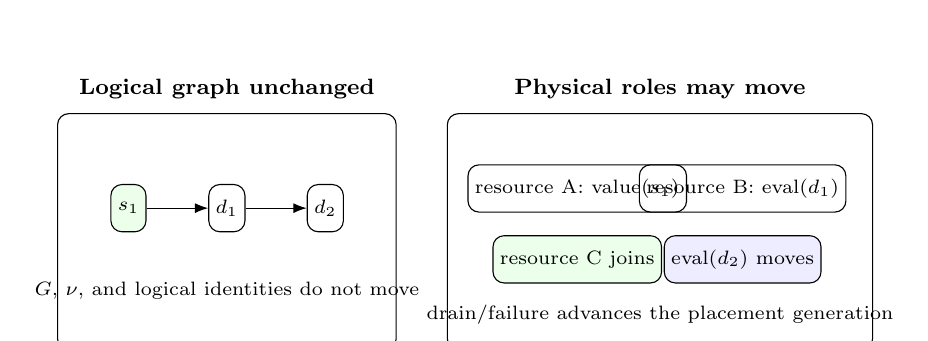
\begin{tikzpicture}[>=Latex,every node/.style={draw,rounded corners,minimum height=6mm,inner sep=2.5pt,font=\scriptsize}]
\node[draw,rounded corners,minimum width=4.3cm,minimum height=3.0cm,label={[font=\footnotesize\bfseries]above:Logical graph unchanged}] (left) at (0,0) {};
\node[fill=green!8] (s) at (-1.25,0.3) {$s_1$};
\node (d1) at (0,0.3) {$d_1$};
\node (d2) at (1.25,0.3) {$d_2$};
\draw[->] (s)--(d1); \draw[->] (d1)--(d2);
\node[draw=none,font=\scriptsize] at (0,-0.75) {$G$, $\nu$, and logical identities do not move};
\node[draw,rounded corners,minimum width=5.4cm,minimum height=3.0cm,label={[font=\footnotesize\bfseries]above:Physical roles may move}] (right) at (5.5,0) {};
\node (r1) at (4.45,0.55) {resource A: $\mathrm{value}(s_1)$};
\node (r2) at (6.55,0.55) {resource B: $\mathrm{eval}(d_1)$};
\node[fill=green!8] (r3) at (4.45,-0.35) {resource C joins};
\node[fill=blue!7] (r4) at (6.55,-0.35) {$\mathrm{eval}(d_2)$ moves};
\node[draw=none,font=\scriptsize] at (5.5,-1.05) {drain/failure advances the placement generation};
\end{tikzpicture}
\caption{Joining, reassignment, graceful drain, and bounded fail-stop recovery change physical placement, not logical identities or dependency meaning.}\label{fig:placement}
\end{figure}
Figure~\ref{fig:placement} summarizes the separation between persistent logical roles and movable physical resources.
\fi

When a definition and one of its premises are on different resources, the dependency becomes a communication obligation. The bounded wire profile carries logical state identity, committed source epoch, placement-role key, placement generation, checksum, and an immutable scalar value. Reliable delivery may be delayed, duplicated, or reordered; a receiver therefore admits a value only for the expected role and current generation. An older epoch is stale, a duplicate same value is harmless, and a different value for the same state/role/epoch is a conflict. The executable placed profile sends every premise through real TCP loopback before evaluation, exercising transport framing, checksum validation, duplicate admission, wrong-role rejection, stale-epoch rejection, and stale-generation rejection without claiming a production multi-host system.

An observation names a logical state rather than a machine. A conforming ingress may return a valid local materialization, retrieve a valid remote materialization, or stabilize the required ancestor region and return its value; these alternatives must agree on the stable logical result.

Each assigned physical role $\ell$ has a placement generation. Work captures a token $(\ell,r,g)$ and may publish only when $\pi_t(\ell)=r$ and $\gamma_t(\ell)=g$. Reassignment, drain, or failure advances the generation so late work from the previous resource cannot publish.

\begin{definition}[Placed-epoch conformance]\label{def:placed}
A physical execution of one finite logical epoch is conforming when transport preserves logical values; every non-discarded derived publication is currently active and ready, equals its local function applied to the committed logical pre-valuation, and carries a current role token; join/reassignment/drain change only physical placement and copies, never $G$, source facts, or logical definition authority; and, after finitely many placement changes, required transport and active logical roles eventually complete.
\end{definition}
\begin{theorem}[Failure-free join/drain transparency]\label{thm:join}
Every conforming placed execution projects, after duplicate and stale physical events are discarded, to a valid sequence of finite frontier-subset transitions. Consequently, after source and placement quiescence, its observable values equal local stabilization.
\end{theorem}
A currently admitted publication is either one legal singleton frontier transition or part of a commuting frontier batch. Join and drain change where later work occurs, not the logical transition represented.

\begin{definition}[Recoverable placed profile]\label{def:recoverable}
Source facts acknowledged as recoverable are durably committed by one declared authority. Pure derived materializations are reconstructible caches. After a finite fail-stop loss, the realization invalidates lost role generations, reassigns roles, restores authoritative sources, marks each lost derived state and its transitive user region as repair obligations, and stabilizes again.
\end{definition}
\begin{theorem}[Finite fail-stop reconstruction]\label{thm:failstop}
For a finite acyclic pure DOC graph, if authoritative source facts survive and remain fixed during the final recovery interval, at least one valid execution resource eventually remains or joins, generation invalidation rejects late failed work, transport eventually succeeds, and no further failure occurs during that interval, reconstruction reaches the same observable stable valuation as local evaluation from those source facts.
\end{theorem}
The replacement begins from the same sources as complete reevaluation. Lost derived states and their user regions are active, so the recovery seed is repair-admissible; Theorem~\ref{thm:finite} gives termination and unique values, while generation checks prevent obsolete candidates from replacing them.

Dependency edges expose potential communication and ready-frontier independence. Placement policy may consider computation cost, value size, update frequency, memory pressure, latency, failure domains, accelerator suitability, and capacity. Adding resources enlarges the physical resource set while leaving the application graph unchanged. The implemented/argued profile covers finite joins, graceful drains, and bounded fail-stop reconstruction under surviving source authority, eventual transport/resource availability, generation admission, and a final quiescent interval. Network partitions, election, quorum, replica consistency, stale-read policy, Byzantine behavior, and irreversible external effects remain explicit distributed-system policy.

\subsection{Distribution, effects, and application structure}
Ordinary DOC programs name logical states and definitions rather than machines, routes, topics, shard identifiers, or worker counts. The placed realization turns remote premise relations into transport obligations and may choose eager propagation, demand-driven stabilization, batching, co-location, or migration without changing the logical graph. When a broker is used only to notify already-known dependents that current state changed, the induced users relation already defines that routing relation. This is deliberately narrower than replacing durable event logs: ordered replay, consumer offsets, audit retention, ingestion buffering, historical queries, and exactly-once irreversible actions are different semantics.

Nondeterministic observations enter as source updates, while recoverable absence or failure may be typed option/result values. Irreversible interaction remains different. A practical boundary separates pure derivation of an intended effect and stable idempotency identity; authorization and ordering policy; durable intent/attempt recording when required; external execution; and durable outcome recording with application-specific retry, deduplication, or reconciliation. A crash after an external system accepted an action but before the committed outcome was recorded leaves uncertainty. Dependency cannot infer authorization, rollback, or external atomicity.

The same finite semantics admits several interpretations. In a compiler, source text $T$ and options $O$ feed parsed declarations $P$, exported interface $I$, diagnostics $D_g$, optimized unit $U$, and generated object $B$. An edit activates only direct users of $T$; if a rebuilt interface is proven equal, users that depend only on $I$ are not activated. In a build system, files/configuration/tool identities/artifacts/results are states and a changed file activates only dependent targets. In a maintained query, base records and parameters are sources and filtered sets, joins, aggregates, and views are derived states. In a long-lived information workflow, evidence, extracted facts, classifications, plans, and reports are logical states; human approval, audit retention, external publication, and nondeterministic tools remain explicit boundaries.

\section{Experimental validation and reproducibility}\label{sec:validation}
\subsection{Runtime conformance}
The executable witness is subordinate to the model: \emph{paper model} $\to$ observable obligations $\to$ runtime refinement, not the reverse.

\begin{definition}[Finite interaction-trace conformance]\label{def:trace}
Let $\eta$ be any finite admissible sequence of committed source batches, stable observations, and immutable graph-version commits beginning from $(G_0,Q_0)$. A physical realization $P$ conforms when
\[
\Obs_P(\eta)=\Obs_{\DOC}(G_0,Q_0,\eta).
\]
The sequence is a mathematical test sequence, not retained application history or a component of $G$ or $Q$. Internal schedules, materializations, cache states, reconstruction steps, placements, and reclamation events may differ.
\end{definition}
Recurrent observations are ordinary observations of epoch-indexed states within a finite demanded prefix.

Application graphs never specify a worker count; experimental limits are supplied externally. Resource join and removal are realization operations over placement. They are not application-level topology instructions.

\subsection{Verification scope}
The native runtime suite contains 36 named conformance suites plus a separate equivalence test for the benchmark generator. Its randomized differential component checks 9,600 update epochs against complete reevaluation, including randomized legal frontier-subset schedules. Twenty repeated optimized runs of the two native test executables completed successfully.

Five independent bounded checkers cover complementary state spaces. The ordinary finite checker enumerates 2,520 Boolean DAGs and 40,320 source epochs. The repair checker covers 512 graphs, 59,904 admissible seeds, 239,616 continued source updates, and 521,584 unique explored configurations. The graph-version checker covers 64 graph shapes and 15,360 commits, including source/derived authority transitions. The duplicate-premise checker covers 84 graphs and 2,592 admissible configurations. The demand/recurrence checker covers 364 demand templates, 21,840 demanded subsets, 364 recurrence templates, 17,472 finite prefixes, 2,912 stopping cases, and duplicate-carry rejection.

These bounded enumerations check initialization, repair admissibility, continued source batches, every nonempty legal subset of each bounded ready frontier, exact and conservative cutoff, locality, schedule agreement, demand restriction, recurrence support, graph-role changes, identifier reorderings, and replacement agreement. They are executable counterexample search over stated finite spaces, not a proof of universal correctness. The high-performance evaluator remains specialized to scalar values; typed immutable objects, eviction, and reconstruction are checked in a separate safe-realization profile. The placed runtime uses real transport but remains a bounded single-coordinator witness, and the finite metatheory is not proof-assistant mechanized.

\begin{table}[t]
\centering\scriptsize
\caption{Mapping from semantic obligations to the executable witness.}\label{tab:witness}
\begin{tabularx}{\textwidth}{@{}p{.21\textwidth}X@{}}
\toprule Model obligation & Witness behavior\\ \midrule
Finite kernel & Optional scalar value plus transient active marker per state; dependency-minimal ready frontier; private complete-frontier evaluation; changed candidates published together.\\
Atomic interaction & Validates a complete source batch before mutation, serializes accepted source epochs, and exposes observations only after stable commit.\\
Schedule independence & Sequential, parallel, randomized, and bounded legal frontier-subset schedules are compared with complete reevaluation.\\
Versioned recurrence & Finite demanded prefixes, forward carry bindings, explicit retention, and a two-counter-machine prefix compared with a direct interpreter.\\
Immutable graph succession & Candidate validation/stabilization, stable-name source carry, compatibility-gated reuse, atomic generation commit, stale-generation rejection.\\
Logical availability & Immutable publications and active-use pins; reconstructible eviction; equal complete reconstruction before observation; reclaim obsolete unpinned objects.\\
Placement/recovery & Generation-bound admission, join/drain, lost-derived reconstruction, and bounded fail-stop recovery from surviving authoritative source facts.\\
Effect boundary & Explicit request, authorization, in-flight uncertainty, outcome recording, and rejection of impossible state transitions without claiming external exactly-once behavior.\\ \bottomrule
\end{tabularx}
\end{table}

\subsection{Performance evaluation}
The benchmark executable checks every DOC output against an independent correctness oracle and exits nonzero on disagreement. Reduction workloads compare against complete serial reevaluation; the financial workload additionally compares against a conventional serial cached segment tree; and the sorting-network workload checks both direct execution of the same Batcher network and \texttt{std::sort}. The benchmarked runtime uses signed 64-bit integer values with exact equality and chooses the complete ready frontier $F=R(A)$; \texttt{DOC\_MAX\_WORKERS} limits participant capacity externally.

The authoritative campaign used GCC 15.3.0 Release on Linux 6.18.53 (x86-64, glibc 2.42) with an AMD Ryzen AI 7 350 w/ Radeon 860M on bare metal. The host exposed 8 physical cores and 16 logical CPUs, with no recorded cgroup CPU quota; Python 3.14.7 and CMake 4.4.2 were recorded. Every reported row used 100 fresh processes plus three unrecorded warmups. Scenario order alternated forward/reverse between samples. Raw measurements are retained in full; a symmetric Tukey 1.5-IQR sensitivity filter supplies a robustness view. The generated report uses a two-sided Student-$t$ interval through 31 observations and the normal approximation above that threshold, so displayed $n=100$ intervals use the latter convention. Participant limits are deliberately capped at 1--4 so the scaling claim remains a bounded single-host result.

A source/reference archive accompanying submission contains the C++20 runtime, registered tests, five bounded model checkers, benchmark driver, raw measurements, statistical summaries, machine record, and both manuscript sources. No external repository access is required for review.

\subsubsection{Workload structure and scheduler granularity}
The 2,048-leaf reduction graph contains 2,048 source states, 2,048 expensive leaf definitions, and 2,047 reduction definitions: 6,143 states and 4,095 derived definitions. Each expensive leaf counts primes in a deterministic interval. The parallel-capacity workload uses 40 sources, 40 expensive leaf definitions, and 39 reduction definitions; its first ready frontier contains 40 independent expensive definitions, each scanning a 25,000-integer interval. The dense cheap negative control uses 4,096 sources, 4,096 identity leaf definitions, and 4,095 sum definitions over 30 full-change epochs. The financial graph contains 24,575 states and 8,191 derived definitions. The sorting workload has 512 sources and a complete Batcher network with 11,520 compare-exchanges represented by 23,040 derived definitions.

\subsubsection{Sparse repair, saturation, and negative control}
\begin{table}[t]
\centering\footnotesize
\caption{Finite-kernel reduction workload on the authoritative bare-metal environment. Timings are raw means over 100 fresh processes; evaluation counts are deterministic.}\label{tab:reduction}
\begin{tabular}{@{}lrrr@{}}\toprule
Scenario & Direct mean & DOC mean & Evaluations\\ \midrule
Cold 2,048-leaf reduction & 351.143 ms & 349.868 ms & 4,095\\
1 changed source & 350.676 ms & 0.661 ms & 12\\
8 changed sources & 351.021 ms & 1.761 ms & 23\\
64 changed sources & 348.163 ms & 11.044 ms & 132\\
512 changed sources & 349.452 ms & 87.671 ms & 1,007\\
2,048 changed sources & 345.352 ms & 346.975 ms & 4,038\\
Dense cheap control (30 epochs) & 0.309 ms & 57.658 ms & 245,730\\ \bottomrule
\end{tabular}
\end{table}
The structural trend in Table~\ref{tab:reduction} is the main result: sparse updates reconsider only changed leaves and ancestors, while dense updates approach complete work. Exact equality cutoff required one producer evaluation and one cutoff in its dedicated microbenchmark. Cold DOC and direct execution are near parity on this expensive reduction, and complete source change also approaches parity. The deliberately cheap dense graph is a negative control: metadata, frontier construction, and synchronization dominate useful arithmetic. The model therefore predicts where work may be avoided, not universal timing improvement.

\iffullvisuals
\begin{figure}[t]
\centering
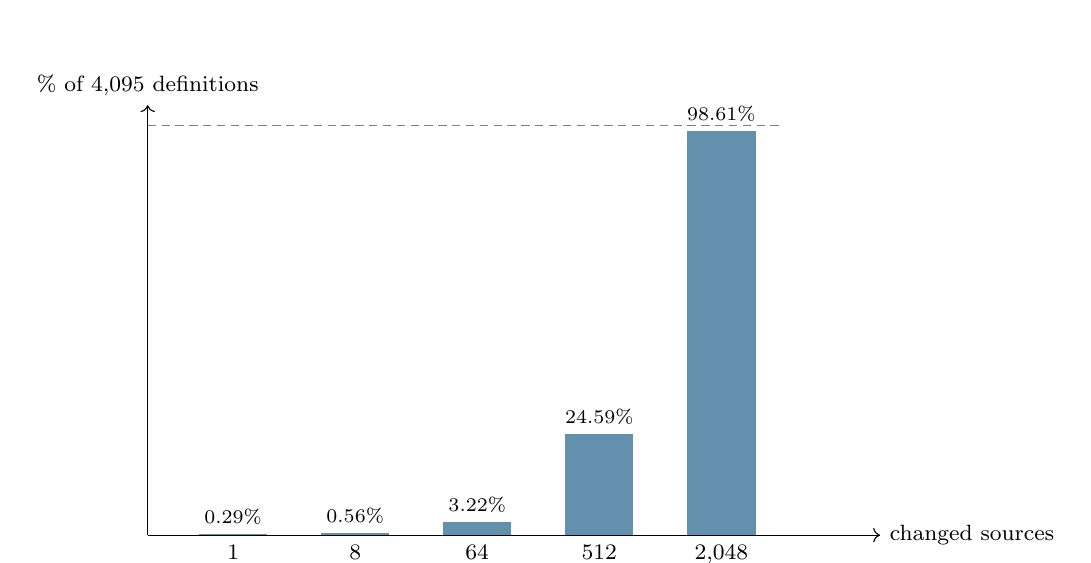
\begin{tikzpicture}[x=1.55cm,y=0.052cm,font=\footnotesize]
\draw[->] (0,0)--(6.0,0) node[right] {changed sources};
\draw[->] (0,0)--(0,105) node[above] {\% of 4,095 definitions};
\foreach \x/\lab/\h in {0.7/1/0.29,1.7/8/0.56,2.7/64/3.22,3.7/512/24.59,4.7/{2,048}/98.61}{
  \fill[docaccent!75] (\x-0.28,0) rectangle (\x+0.28,\h);
  \node[below] at (\x,0) {\lab};
  \node[above,font=\scriptsize] at (\x,\h) {\h\%};
}
\draw[densely dashed,gray] (0,100)--(5.2,100);
\end{tikzpicture}
\caption{Repair work grows with update density. Bars show selected definitions as a fraction of the 4,095 derived definitions; equality cutoff leaves the full-change row slightly below 100\%.}\label{fig:repair-density}
\end{figure}
Figure~\ref{fig:repair-density} visualizes the same deterministic evaluation counts reported in Table~\ref{tab:reduction}.
\fi

\subsubsection{Externally granted parallel capacity}
\begin{table}[t]
\centering\footnotesize
\caption{Ready-frontier scaling under externally granted participant limits on one bare-metal host.}\label{tab:parallel}
\begin{tabular}{@{}rrr@{}}\toprule
Participants & Raw mean (95\% CI) & Raw speedup\\ \midrule
1 & 270.151 ms (267.988--272.314) & 1.000$\times$\\
2 & 140.117 ms (139.015--141.219) & 1.928$\times$\\
3 & 97.909 ms (96.727--99.092) & 2.759$\times$\\
4 & 76.228 ms (75.499--76.957) & 3.544$\times$\\ \bottomrule
\end{tabular}
\end{table}
The single-host result reaches 3.544$\times$ at four participants, corresponding to about 88.6\% parallel efficiency relative to ideal four-way scaling. Across the measured one-to-four-participant range, each successive increase retains approximately 95--96\% of the corresponding ideal incremental scaling step, with no abrupt degradation over the observed range. This empirical regularity is not extrapolated beyond four participants, and the experiment does not identify the source of the residual gap. Future work can test whether topology-aware placement, workload granularity, or runtime refinements can reduce it toward negligible levels. The first frontier contains 40 independent expensive leaves, enough coarse work to amortize runtime overhead. The experiment contains no inter-host transport and supports only the claim that a dependency-minimal frontier can consume externally granted local capacity without a worker count in the program.

\iffullvisuals
\begin{figure}[t]
\centering
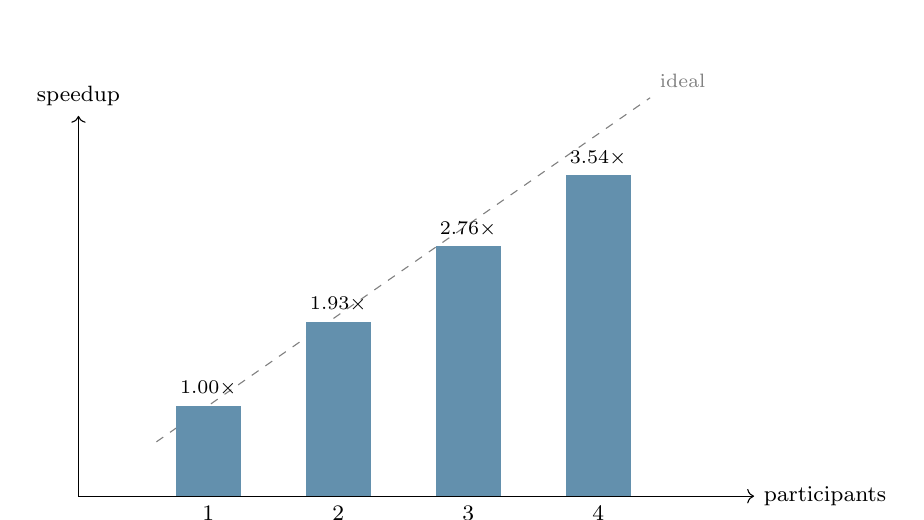
\begin{tikzpicture}[x=1.65cm,y=1.15cm,font=\footnotesize]
\draw[->] (0,0)--(5.2,0) node[right] {participants};
\draw[->] (0,0)--(0,4.2) node[above] {speedup};
\draw[dashed,gray] (0.6,0.6)--(4.4,4.4) node[above right,font=\scriptsize] {ideal};
\foreach \x/\p/\h/\lab in {1/1/1.000/{1.00$\times$},2/2/1.928/{1.93$\times$},3/3/2.759/{2.76$\times$},4/4/3.544/{3.54$\times$}}{
  \fill[docaccent!75] (\x-0.25,0) rectangle (\x+0.25,\h);
  \node[below] at (\x,0) {\p};
  \node[above,font=\scriptsize] at (\x,\h) {\lab};
}
\end{tikzpicture}
\caption{Single-host ready-frontier speedup. The result demonstrates use of granted local capacity for a coarse frontier; it is not evidence of distributed scalability.}\label{fig:parallel-speedup}
\end{figure}
Figure~\ref{fig:parallel-speedup} shows the bounded scaling curve corresponding to Table~\ref{tab:parallel}; no extrapolation beyond four participants is made.
\fi

\subsubsection{Realistic persistent financial projection}
The financial workload models 4,096 business units. Each unit has four source cells and one deterministic 360-period fixed-point cash-flow projection; a balanced tree consolidates unit values. Each changed unit updates revenue and payroll sources. Complete serial reevaluation, a conventional serial cached segment-tree repair, and DOC must produce the same total.
\begin{table}[t]
\centering\footnotesize
\caption{Financial projection workload; all implementations are checked for equal output.}\label{tab:financial}
\begin{tabular}{@{}rrrrr@{}}\toprule
Changed units & Full mean & Cached mean & DOC mean & DOC evals\\ \midrule
1 & 7.845 ms & 0.00240 ms & 2.226 ms & 13\\
64 & 7.890 ms & 0.1284 ms & 2.405 ms & 133\\
1,024 & 7.896 ms & 2.045 ms & 4.398 ms & 2,049\\ \bottomrule
\end{tabular}
\end{table}
DOC is faster than complete reevaluation for all three displayed update sizes, but the specialized cache is substantially faster than generic DOC repair. For one changed unit, DOC takes about 28\% of full reevaluation time yet about 929 times the cached update time; at 64 units the cached baseline is about 18.7 times faster than DOC; at 1,024 units it remains about 2.15 times faster. The useful conclusion is workload-specific: generic overhead is justified only when reusable semantics, dynamic affected-region discovery, graph evolution, conformance properties, or a common runtime mechanism are worth more than a hand-specialized incremental path.

\subsubsection{Fine-grained graph negative case}
A 512-input Batcher sorting network contains 11,520 compare-exchanges represented by 23,040 derived definitions and 23,552 total states. Sparse updates avoid many definitions and expose equality cutoffs, but direct complete network execution is far faster: raw DOC update means range from 10.26 to 11.11 ms, while direct update means range from 0.0524 to 0.0832 ms. The DOC/direct ratio ranges from about 128$\times$ to 211$\times$. At full change, all 23,040 definitions execute and no cutoff remains. This negative case shows that exposing a dependency at every comparator can make the logical graph useful for reasoning while making runtime granularity uneconomic; fusion, batching, or specialized operators would be required for a competitive implementation.

These measurements support only conformance and workload-specific cost-shape claims. They do not establish universal speedup, distributed scalability, accelerator efficiency, or constants independent of hardware. Stronger scaling claims require dedicated many-core and multi-host experiments, not extrapolation from Table~\ref{tab:parallel}.

\section{Limitations}\label{sec:limitations}
\begin{enumerate}[label=\arabic*.]
\item \textbf{Finite acyclic theorem.} The central theorem covers finite acyclic programs. Versioned recurrence supplies temporal repetition and ordinary partial computation, but same-epoch cyclic equations require separately stated order, convergence, and observation semantics.
\item \textbf{Equality and function contracts.} Sound cutoff, total deterministic definitions, stable-name compatibility, and semantic keys are supplied by a compiler, builder, or application contract; the runtime cannot decide arbitrary function equivalence.
\item \textbf{Policy-dependent physical behavior.} Placement, routing, replica authority, partition handling, retention, compaction, checkpoints, quotas, and irreversible-effect recovery are not determined by the logical kernel.
\item \textbf{No universal memory or performance bound.} Logically rooted recurrence or audit history may grow without bound. Direct or specialized incremental execution may outperform the generic runtime, especially for dense or fine-grained work.
\item \textbf{Evidence limits.} The finite metatheory is not proof-assistant mechanized. Exhaustive checking is bounded. The physical witness is a bounded single-coordinator implementation, and the reported scaling measurements are limited to participant counts 1--4 on one bare-metal host; they do not establish many-core or multi-host scaling.
\end{enumerate}

\section{Related work}\label{sec:related}
Dependency-oriented evaluation has several established lineages. Kahn process networks provide deterministic semantics for communicating processes \cite{kahn1974}. Attribute grammars attach semantic values to syntactic structure and expose dependency relations; Knuth established the framework \cite{knuth1968,knuth1971correction}, and Demers, Reps, and Teitelbaum studied incremental reevaluation for syntax-directed editors \cite{demers1981}. INC is an early language explicitly designed for incremental computations \cite{yellin1991}. These works establish that dependency structure and incremental maintenance are not new ingredients of DOC.

The closest comparison is self-adjusting computation. Acar's model represents computations with dynamic dependence graphs and uses change propagation after external changes \cite{acar2005}. Parallel self-adjusting computation develops additional machinery and work/span analysis for parallel change propagation \cite{anderson2021}. Adapton combines incremental computation with demand and introduces a demanded computation graph plus an explicit observer boundary \cite{hammer2014adapton}. DOC makes a different representational choice: the graph of logical state identities and definitions is declared as the persistent program for one graph version, while transient repair state is represented separately by $A$ and the finite repair relation acts only on dependency-minimal active definitions. This is a distinction in factorization and proof boundary, not a claim that change propagation, memoization, demand, or parallel dependency processing originated here.

Build systems provide another close comparison because they preserve results across repeated changes. \emph{Build Systems \`a la Carte} factors build systems into tasks plus scheduling and rebuilding components and compares static and dynamic dependency strategies \cite{mokhov2018}. DOC instead fixes a language-neutral state/definition representation for the finite theorem and derives readiness from the current active set. Build-specific dependency discovery, command effects, artifact hashing, and failure policy remain outside the pure theorem.

Incremental dataflow systems occupy a richer iteration/distribution point. Differential dataflow associates state and updates with partially ordered logical versions and retains indexed differences for incremental iterative computation \cite{mcsherry2013}. Naiad's timely dataflow is a distributed cyclic dataflow model with logical timestamps and progress coordination \cite{murray2013}. DOC deliberately does not place those mechanisms in its finite acyclic kernel; recurrence is forward-linked finite epochs while placement and transport are realization contracts. This simplifies the finite theorem but gives up native cyclic/timestamp semantics.


Static differentiation derives change functions for higher-order programs \cite{cai2014}; materialized-view maintenance derives incremental updates for database views \cite{blakeley1986}; and spreadsheet systems provide a familiar dependency-maintained interface, with recent work on scalable incremental spreadsheet applications \cite{hadar2023}. Persistent incremental traces also create storage-management problems; Hammer and Acar study memory management specifically for self-adjusting computation \cite{hammer2008memory}. These comparisons reinforce the narrower positioning: DOC contributes neither a new general change calculus nor a domain-specific optimal incremental algorithm.

The assessable technical claim is limited to the finite factorization proved in Theorem~\ref{thm:finite} and its explicitly separated extensions: a persistent typed logical-state graph $G=(S,\Delta)$; retained valuation $\nu$; transient repair-obligation set $A$; dependency-minimal ready states; arbitrary nonempty ready-frontier subset selection from one settled pre-state; atomic publication of changed conclusions; and a one-way sound cutoff predicate whose always-false implementation remains correct. The experiments ask whether this factorization is coherent, executable, and useful as a generic semantic boundary---not whether it dominates specialized incremental systems.

\section{Conclusion}
The finite model makes dependency structure, retained values, and repair obligations explicit through $G=(S,\Delta)$ and $Q=(\nu,A)$. A stable valuation agrees with current sources and every required definition. A source change adds induced users to the repair obligations. One transition selects any subset of the dependency-minimal active frontier, evaluates it from a common settled pre-state, and publishes complete candidates together. Candidates not proven equal propagate; a sound equality proof stops the wave.

The finite kernel deliberately contains only the persistent graph, retained valuation, repair obligations, and transition relation. Recurrence, graph replacement, and physical placement are separate layers with additional assumptions. Publication, reclamation, transport, authority, reconstruction, and effects remain explicit contracts rather than consequences silently attributed to the finite theorem. DOC does not claim universal speedup or distributed-systems guarantees. Its contribution is the specific finite repair semantics proved here, together with separately stated extension and realization contracts and an executable implementation that tests those boundaries.

\bibliographystyle{unsrt}
\bibliography{references}
\end{document}
